\documentclass{./llncs2e/llncs}
\usepackage{graphicx}
%%%%
\usepackage{fixltx2e}
%%%%
\usepackage{mathtools}
%%%%
\usepackage[nolist,nohyperlinks]{acronym}
%%%%
\usepackage[section]{placeins}
%%%% Maintain images and tables within their respective sections
\usepackage{float}
%%%%
\usepackage[utf8]{inputenc}
%%%% Declare that we're using utf8 encoding
\usepackage{listings}
%%%% Include package for listings


% 
% Change the margins
% 
% \usepackage[margin=2.9cm]{geometry}

\begin{document}
\title{Your Thesis title}

\subtitle{Your Thesis subtitle}
\author{Pedro Alfaiate, pedro.alfaiate@tecnico.ulisboa.pt}
\institute{Instituto Superior Técnico}

\maketitle

%----------------------------------------------------
%NAVabstract
\begin{abstract}

\end{abstract}
%----------------------------------------------------
%NAVkeywords
\begin{keywords}

\end{keywords}
%----------------------------------------------------
%NAVintroduction
\section{Introduction (2/3pgs)}
%TODO: Introduce the well established tools (ex: cads) that architects and designers use in their work.
%TODO: Introduce the concept of Generative Design approach so it can be used later. It isn't known to everybody.
%%%%Writing a program with a programming language is a great way to structure our thoughts. 

%----------------------------------------------------
%NAVobjectives
\section{Objectives (1pg)}
The aim of this project is to provide architects and designers interested in creating 3D models with an environment that fosters the Generative Design approach while being accessible wherever they are working.

%Why does it need to be accessible wherever the architect is?
Architects imagine buildings and will have to move their ideas to outside of their heads wherever they are; if they don't, they might forget them forever. We have to provide a means to translate ideas and it has to be accessible wherever they are.\textsuperscript{citation needed}
%TODO: Come up with an alternative to "translate ideas". Maybe "express ideas".

How can we provide a means to translate ideas? We make them translate the idea into a program, we encourage them to use Generative Design.

When architects look for an environment to program they aren't looking for a software development \ac{ide} like Eclipse or Visual Studio. They only need an environment where they can write their program and see the results. All they want is accessible programming languages and environments.

%TODO: Rephrase the following paragraph since the well established tools were introduced earlier.
There are many well established tools that architects use to translate their ideas; if we're going to come up with a solution that can rival them than it must be as easy to try out as possible; and be able to integrate with them.
%Should I say how it integrates with them? Which is by offering the possibility of producing effects on their current tools, more specifically the CADs they use.

Summing up, the result of this project should:
\begin{enumerate}
	\item Be accessible wherever the architect is working; \label{obj:access}
	\item Support the Generative Design approach; \label{obj:gen-design}
	\item Be as easy to try out as possible -- without a middle step to install it; \label{obj:no-install}
	\item Integrate with the tools that architects and designers already use.\label{obj:inter-op}
\end{enumerate}


%----------------------------------------------------
%NAVrelatedwork
\section{Related Work (~17pgs)}
In this section we start by describing work done on making programming accessible to everyone and extract the principles that should be followed to achieve it.

We move on to present some of the current widely used solutions -- or environments -- in the Generative Design community and evaluate their conformance with the principles defined earlier.

\subsection{Making Programming Accessible}
Making programming accessible to everyone has been an active area of research for many years. Some examples of programming languages designed with introducing people to programming were Logo\cite{papert1999logo} -- where the programmer explains the meaning of new words to a turtle -- and Smalltalk\cite{goldberg1983smalltalk} -- where the programmers expresses the way a group of objects exchanges messages to solve a problem. Their authors are great defenders of the notion that learning how to solve/understand problems with a computer is a greater way of learning since it is a dynamic medium. An example of that is the Dynabook\cite{Kay:2011:PCC:800193.1971922}, a handheld computer prototype for children where programming is an important activity.

Writing a program in a programming language can be difficult even if it was designed to be easy to use. When a programming language is coupled with an environment specifically designed for it the programming experience improves drastically. In his essay\cite{victor2012learnable}, Bret Victor described design principles over systems for learning programming; we will enumerate and describe each one of them.

\subsubsection{Learnable Programming\cite{victor2012learnable}}
In this essay, Bret Victor starts by stating what the goals of a programming system should be: it should ``support and encourage powerful ways of thinking''; and it should ``enable programmers to see and understand the execution of their programs''.

%TODO: Change the type of discourse to a "synthesis" of what Bret Victor said instead of a "narration" of how he said it in his paper.
He then states that a programming system has two parts -- the \emph{programming environment} which is installed on the computer; and the \emph{programming language} which is installed on the programmer's head -- and then presents the design principles for those parts.

The principles for the environment state what it should allow the programmer to do. The environment should allow the programmer to:
\begin{enumerate}
	\item \label{lp:env:read} read the vocabulary 
	\item \label{lp:env:flow} follow the flow
	\item \label{lp:env:state} see the state
	\item \label{lp:env:react} create by reacting
	\item \label{lp:env:abstr} create by abstracting
\end{enumerate}

The principles for the language state what it should provide. It should provide:
\begin{enumerate}
	\item \label{lp:lang:id} identity and metaphor
	\item \label{lp:lang:decom} decomposition
	\item \label{lp:lang:recom} recomposition
	\item \label{lp:lang:read} readability
\end{enumerate}

%TODO: Change the type of discourse.
These principles are then further explained following the same order. When talking about the principles over the environment, Bret gives examples that follow each principle; those examples aren't included here since they are solutions to a specific case. When talking about principles over the language, he gives examples of languages that follow and don't follow -- and how -- each principle; those are also not included here.

The environment should allow the programmer to \emph{read the vocabulary} so that the he can quickly shift his attention to ``how the steps are weaved together''. That is, as he is reading, the environment should make it easy to understand what each word means; each word's meaning should be made clear in an appropriate context -- or more if necessary.
%How can I say that the environment can use any means necessary to achieve it?

The environment should allow the programmer to \emph{follow the flow} so that he more easily understands ``how the steps are weaved together''. Instead of just showing the code and the result of its execution, the environment must show the execution of the program and let the programmer explore it in various meaningful granularities -- from different perspectives.

The environment should allow the programmer to \emph{see the state} of the program -- be it explicit, as local variables, or implicit, as library state -- so that he can feel how it changes with the execution of the program. The environment must show the state as it changes with the execution and must show meaningful comparisons over the execution -- i.e., if the it represents a color then show it as colors; if it represents a number then show it as numbers.
%Every line of code changes something be either by returning or by having side-effects.

The environment should allow the programmer to \emph{create by reacting} to the environment so that he can ``start with something, than adjust until it's right''. To make it possible, the environment must make it easy to experiment; it must make trying/adding things as fast as the programmer can think of them and also make what can be done obvious. Bret Victor clearly states that this should be like painting. When the user tries things, he doesn't completely know what he's going to get; if what he gets is not right he changes it.

The environment should allow the programmer to \emph{create by abstracting} parts of the program so that he can start by writing a concrete case, then generalizing it. The environment must ``provide ways to gradually and seamlessly transitioning constant expressions'' and also ``provide ways of using those variable expressions at a higher level''. In other more general words: make it easy to generalize using the language's decomposition mechanisms. 

The language should provide a good \emph{identity and metaphor} so that the programmer can easily relate to the program he is writing. These provided enable the programmer to use his knowledge about the world to solve the problem he is trying to solve by writing a program in the language. 

The language should provide \emph{decomposition} so that the programmer can ``breakdown the program into ``mind-size bites''''. It should encourage him to decompose the problem because decomposing is essential for understanding it.

The language should provide \emph{recomposition} so that the programmer can safely reuse parts. It should encourage him to ``grab parts of other programs, assemble them together, modify them, build on top of them'' thus ``giving him the initial material to ``create by reacting''''.

The language should provide \emph{readability} so that the programmer can ``look at a line of code and know what it means''; the meaning of a line of code shouldn't be ambiguous. Its syntax and names matter, i.e. the syntax should provide context to its elements and the names should clearly pinpoint what they represent within their context. It should be readable even without a fancy programming environment.

\subsubsection{Processing\cite{reas2007processing}}
Processing is a programming language and a development environment aimed at ``promoting software literacy in the visual arts and visual literacy within technology''.\footnote{www.processing.org} It has an heavy focus on encouraging interaction between its users and so has attracted a big community.\textsuperscript{citation needed}

Processing makes it easy to start writing programs that produce visual output. The only step required to start using it is the download and installation of one of its releases. After installation one can start the \ac{pde} and start writing a new program, or a \emph{sketch} as it is referred within Processing. Its website also provides a set of tutorials to help users learn how to use it.

Being aimed at producing visual output and given its success by the size of its community, it makes sense to analyze it.

We start by analyzing its programming language, then move to its development environment and finish by evaluating it against \emph{our learnable programming principles}.

%\subsubsubsection{Processing's programming language}
Processing's programming language aims to provide Java-style programming while making it easy to quickly write functioning programs. 

Every program written in Processing is called a \emph{sketch}. All \emph{sketches} are stored in a \emph{sketchbook}.

A \emph{sketchbook} has a set of resources, such as images or videos, that can be used by \emph{sketches} that are stored in it.

A \emph{sketch} is a list of instructions to draw something. Some examples of instructions are drawing a shape, like a rectangle, changing the colors used for drawing lines or filling shapes, and changing the color of the background.

To simplify the \emph{sketch}, named functions can be defined to group instructions. These functions can then be used as instructions throughout the rest of the \emph{sketch}.

A \emph{sketch} can be a static sketch or a dynamic sketch. A static sketch produces a static image while a dynamic sketch produces a series of images. A dynamic sketch includes at least a list instructions of what to do to draw each image; it can also include instruction of what to do to respond to input from the viewer of the \emph{sketch}.

\begin{lstlisting}[caption={A simple Processing sketch},label={lst:simple:processing},language=Java]
//Hello mouse.
void setup() {
    size(400, 400);
    stroke(255);
    background(192, 64, 0);
}
 
void draw() {
    line(150, 25, mouseX, mouseY);
}
\end{lstlisting}

The code in \ref{lst:simple:processing} shows a simple \emph{sketch} with the typical \emph{sketch} structure. The \emph{sketch} draws a white line from one point to the mouse's position. It defines the function ``setup'' and  ``draw'' that specify how to setup for drawing and specify how to draw each image. The ``setup'' is run once when the sketch is started and ``draw'' is repeatedly run afterwards.

%\subsubsubsection{Processing's programming environment}
The \ac{pde} is shown in figure \ref{fig:proc:dev:env}. It is a code editor dedicated to writing Processing \emph{sketches}. It supports common tasks performed while writing Processing them such as running the currently opened \emph{sketch}, adding/creating resources to the \emph{sketchbook} or exporting \emph{sketches} as executables for several platforms. It also enables the use of multiple files to structure the \emph{sketch's} code.

The \ac{pde} only aims to be an introductory environment for programming. It doesn't replace an advanced software development environment.

\begin{figure}
  \centering
  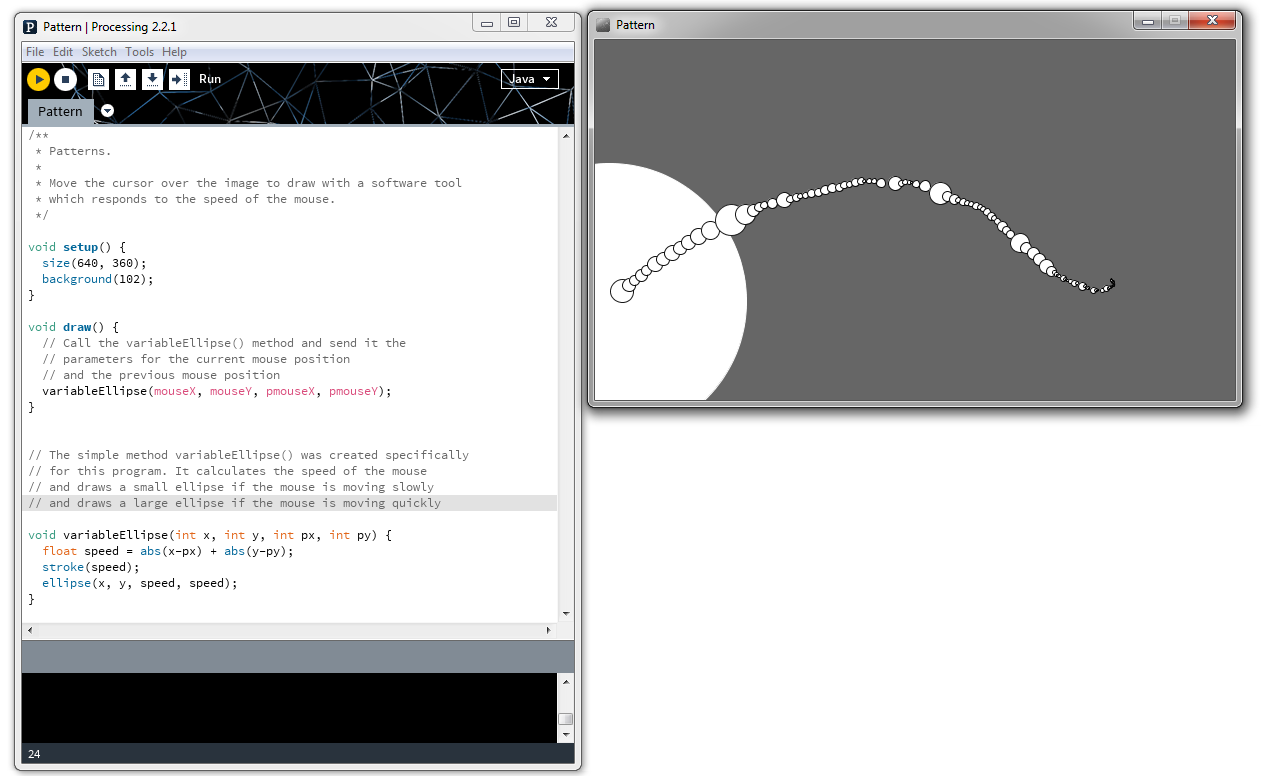
\includegraphics[width=1.0\textwidth]{img/proc_dev_env}
    \caption{On the left: The \ac{pde} displaying an example \emph{sketch} while it is being run. On the right: The drawing window to which the \emph{sketch's} instructions are applied.}
  \label{fig:proc:dev:env}
\end{figure} 

\subsubsection{Processing vs Programming for Everyone}
%This is a comparison with Java. It can be seen as a limitation.
Looking at the code in \ref{lst:simple:processing} also reveals the language's resemblance with Java. The same code fragment in Java declares two methods named ``setup'' and ``draw'' that return nothing; both methods belong to whatever class they happen to be inside of; and both have a list of statements to be executed sequentially when they are invoked. Processing's instructions, functions and sketches map to Java's statements, methods and classes.
%Classes inside sketches are mapped into inner classes.

%Describe what the language and the environment lack to improve the programming experience for its users and uses (arts). 
	%Describe how it is just a quick start package for graphics programming in Java. 
	%Describe how the environment not only lacks a debugger but also doesn't give proper error messages when something fails and doesn't provide other ways to follow the program execution.
%Describe how the environment fails to be a better environment than those used in industry software production (like Eclipse).
	%Describe how its users are required to look for documentation when programming.
	%Describe how little feedback the environment provides. E.g. he has to run the sketch to see if it compiles and runs as he expects. This blocks creation by reaction.
	%Describe how trying to hide Java doesn't make it a better language for learning or producing art. For doing more advanced things, Processing still requires the programmer to know Java; why not learn Java straight away? Processing tries to hide Java's metaphors, its objects; bad idea. (Scala does a better job, I suppose)

\subsubsection{Impromptu\cite{sorensen2005impromptu}}
Impromptu is a programming environment developed to explore manipulation of musical structure in live performance; an \ac{ide} for musicians and sound artists.

%What is live-performance?
In the case of Impromptu, live performance takes place as live programming the algorithms that produce the sounds of the music.

%What does it provide to support live-performance?
To produce live programming Impromptu brings together four components: an audio synthesizer, a real-time scheduling engine, a Scheme interpreter and an \ac{ide}. The first three components make up the runtime environment while the last provides an interface to it. 

%Describe live programming experience of impromptu.
The usage of Impromptu revolves around using its \ac{ide} to send code to the Scheme interpreter. The code can schedule audio to be played later, schedule functions to run later, define or redefine functions and ``variables''. 
One can use Impromptu to incrementally build an algorithm that produces music. He writes small parts of the algorithm, sends them to the interpreter and then uses those parts to build bigger parts. If not satisfied with a part, he can change its code and send it again to the interpreter.


%Describe it as a creative tool. As a try of bringing live coding back to the stage (it states that it happened during late 80s and early 90s). It states that live coding performances are extensions to what is called laptop performances.
%Describe it as being a tool for people interested in making music.  probably have experience with synthesizer software but little programming experience.
%Maybe include link to live performance video.

\subsection{Wrapping Up}
%Summarize the parts of the related work that were major influences of the proposed architecture.

%----------------------------------------------------
%NAVarchitecture
\section{Architecture (2/3pgs)}

%----------------------------------------------------
%NAVevaluation
\section{Evaluation (1/2pgs)}

%----------------------------------------------------
%NAVconclusions
\section{Conclusions}

%----------------------------------------------------
%NAVappendix
\newpage
\appendix
\section{Appendix}
\label{sec:attachments}

%----------------------------------------------------
%NAVacronyms
\begin{acronym}
\acro{ide}[IDE]{integrated development environment}
\acro{pde}[PDE]{Processing development environment}
\end{acronym}

% 
% Bibliography
% 
\bibliographystyle{plain} 

% replace example.bib with your .bib
\bibliography{report} 

\end{document}